\chapter{\textit{Archipelago}}
The game as it is explained in the following section is the result of the design and development process explained in chapters \ref{sec:dev} and \ref{sec:tech} of this paper. Because this prototype is the one covering the largest \textit{scope} among all the prototypes created during this project, it deserves its own section of the report to be explained in details along with the analysis process of the results.
 
This playtest was performed at the end of the development and should answer all the questions raised when implementing PCG-based mechanics into hybrid games. Since the game has been thought from the beginning as an experimental concept, it is expected that the answers provided by the different prototypes will transcend the project presented in this paper. This means that the results that will be presented here will contribute to the exploration of making hybrid games in various ways: the successful design choices must be situated in their particular context, to recognize the patterns that support the hybrid nature of the gale; using the same approach, the experimentations that did not provide the expected results will also be analysed.
\section{The Final Prototype}
\label{sec:finalproto}
The first important thing to know about the final version used to playtest is that it was modified in order to cover aspects that were not working as intended. The following section will first present a simple version rules as they were conceived; another paragraph will be dedicated to explain why these final modifications were necessary for the sake of the paper. Refer to appendix \ref{sec:rules} to see the detailed rules of the game.

\subsection{The components}
Setting up the board is the beginning of every tabletop game. The board is to be placed on the surface area that the players are using, i.e. a table, and the starting conditions, like the initial resources the players have, will be distributed onto the board. Next step is to assign the \textit{Crew Member} tokens to the players. Each player will have their own color on their own tokens and the color itself is arbitrary: it has no relevant meaning to the game itself, rather than making it easier for the players to know which one is theirs.
When the assigning of the player tokens has been done, and the board has been placed, if the game is played by new players, the next step will be to read through the rules of the game, and to have one of the players read out loud and explain the different phases and the possible actions that can be done, along with the costs and rewards of said actions. If this is not done during the start-up of the game, it can also be done at runtime, as there is no set timer within the application, and the players can take the time they need and refer to the rules.
\subsubsection{The Board}
The following paragraph is a description of the physical board and its components. In figure \ref{fig:compo} are the board used and the tokens the players interact with.
\begin{figure}[!ht]
   \centering
   \begin{subfigure}[b]{\textwidth}
       \includegraphics[width=\textwidth]{Images/Board.png}
       \caption{The board of the final tested version of \textit{Archipelago} explained.}
       \label{fig:boardfinal}
   \end{subfigure}
   \begin{subfigure}[b]{\textwidth}
   \centering
       \includegraphics[scale=0.65]{Images/tokens.png}
       \caption{The tokens used in the final version of \textit{Archipelago}.}
       \label{fig:tokens}
   \end{subfigure}
   \caption{The analogue components used to play \textit{Archipelago}.}
   \label{fig:compo}
\end{figure}

When starting the game and placing the board, all the players have available 2 \textit{Crew Member} tokens. The \textit{Cargo Hold} contains 4 \textit{Scrap} tokens, and 1 \textit{Alchemy Point}. The castle itself will start off with 3 \textit{Crystal charges} which powers the \textit{Crystal} at level 1. In order to get to level 2, the players will need to acquire another crystal piece. Upgrading the crystal also enlarges the \textit{Cargo Hold}, which can then contain more \textit{Scrap} and \textit{Alchemy Points}.

The \textit{Construction} box is used to place the resources that were spent during the management phase, so they are separated from the \textit{Cargo Hold} - allowing for more clarity when taking decisions. The \textit{Event} box is used to remember which resources are spent during events. 

Finally, the \textit{Allies} box is used to place the \textit{Faction} card of the faction(s) allied with the players. The allied faction being an important parameter in the procedural generation of the events, it was important that players could always remember who they are allied with. 
\subsubsection{The Application}
As the application is started, the players are presented with the layout of the map. In the center is the castle, as is being represented by the physical board on the table. To move around in the world, all that needs to be done, is to click on an island that is within the ring around the castle, which indicates the travel distance possible for the castle each turn. Once an island is clicked on, a travel confirmation dialogue box will appear, and the players will have to confirm that they do indeed wish to travel there.
\subsection{Phase 1 - Castle Management}
\label{sec:p1}
Before the players have to travel around the world within the app, they have the first phase on the board. This phase is called the \textit{Management Phase}. In this phase, the players can upgrade, repair and expand their castle by building more rooms.

\begin{figure}[!ht]
    \centering
    \includegraphics[scale=0.5]{Images/rooms.png}
    \caption{The different types of rooms.}
    \label{fig:roomtype}
\end{figure}

In figure \ref{fig:roomtype} are the different types of rooms available for construction. Building a standard room (taking only one construction space) costs 2 \textit{Scrap} tokens, and 1 \textit{Crew Member} has to be assigned to the construction. This \textit{Crew Member} will not be available during the next phase of the game.
There is no limit for how much players can do during this phase, other than what the players themselves have the resources for. A room can be damaged after an event. In that case, the players flip the room and it is not usable until it is repaired for 1 \textit{Alchemy Point} and 1 \textit{Scrap} per tile occupied by the room. A destroyed room has to be rebuilt from the beginning.



During the \textit{Management Phase}, the players can also assign \textit{Crew Members} to a room that is already built. All the rooms have different effects:
\begin{labeling}{\textbf{Mechanic's Workshop}}
\item[\textbf{Mining room}] The crew members assigned to this room will gather \textit{Scrap}. The amount of \textit{Scrap} gathered per \textit{Crew Member} assigned depends on the level of the room.
\item[\textbf{Alchemy Lab}] The \textit{Alchemy Lab} is used on the board to gather \textit{Alchemy Point}. The amount of \textit{Alchemy Points} gathered per \textit{Crew Member} assigned also depends on the level of the room.
\item[\textbf{Mechanic's Workshop}] The \textit{Mechanic's Workshop} is used to repair damaged rooms. When a room is damaged, the players assign 1 \textit{Crew Member} to the mechanic's workshop to repair it. It takes one turn per tile occupied by the damaged room to repair it. Upgrading the mechanic's workshop increase the speed at which a room is repaired.
\item[\textbf{Chapel}] The \textit{Chapel} is used to heal \textit{Crew Members} that got injured during an event. It costs 1 \textit{Alchemy Point} and takes one turn to heal an injury. The number of \textit{Crew Members} that can be healed per turn depends on the size of the \textit{Chapel}.
\end{labeling}

When two rooms of the same type are built next to each other, they can be merged, thus accessing the next level and becoming more powerful (see figure \ref{fig:merge}). Upgrading a room also requires 1 \textit{Alchemy Point} per tile occupied by the upgraded room. Again, this will require a player to temporarily set a crew inactive, as it has to build the room. It is worth noticing that the crystal as to be upgraded in order to merge rooms.

\begin{figure}[!ht]
    \centering
    \includegraphics[scale=0.5]{Images/merge.png}
    \caption{The room merging system. In the top left corner of each tile, the players can see the \textit{Crystal}'s level required to build the room.} 
    \label{fig:merge}
\end{figure}
\subsubsection{Collaboration and Mastery}
The merging mechanic introduces specialization or \textit{Mastery}. In \textit{Archipelago}, all players can perform almost all the basic actions in the game. There is no specific skill related to a specific role. However, a player alone cannot perform all the actions required by the game at the same time: the amount of actions that a player can perform is directly related to the number of \textit{Crew Members} that this player commands. Therefore, it is important to encourage the players to split the tasks among them. The tasks can be divided into several groups that are related to the type of rooms that can be built in the castle. 

When a players spends one of her \textit{Crew Member} to merge a room, that player gain a \textit{Specialization token} of the same type as the room that was upgraded. There are 3 different levels per specialization, depending on the size of the room that has been upgraded after merging (see figure \ref{fig:spec}). 

\begin{figure}[!ht]
    \centering
    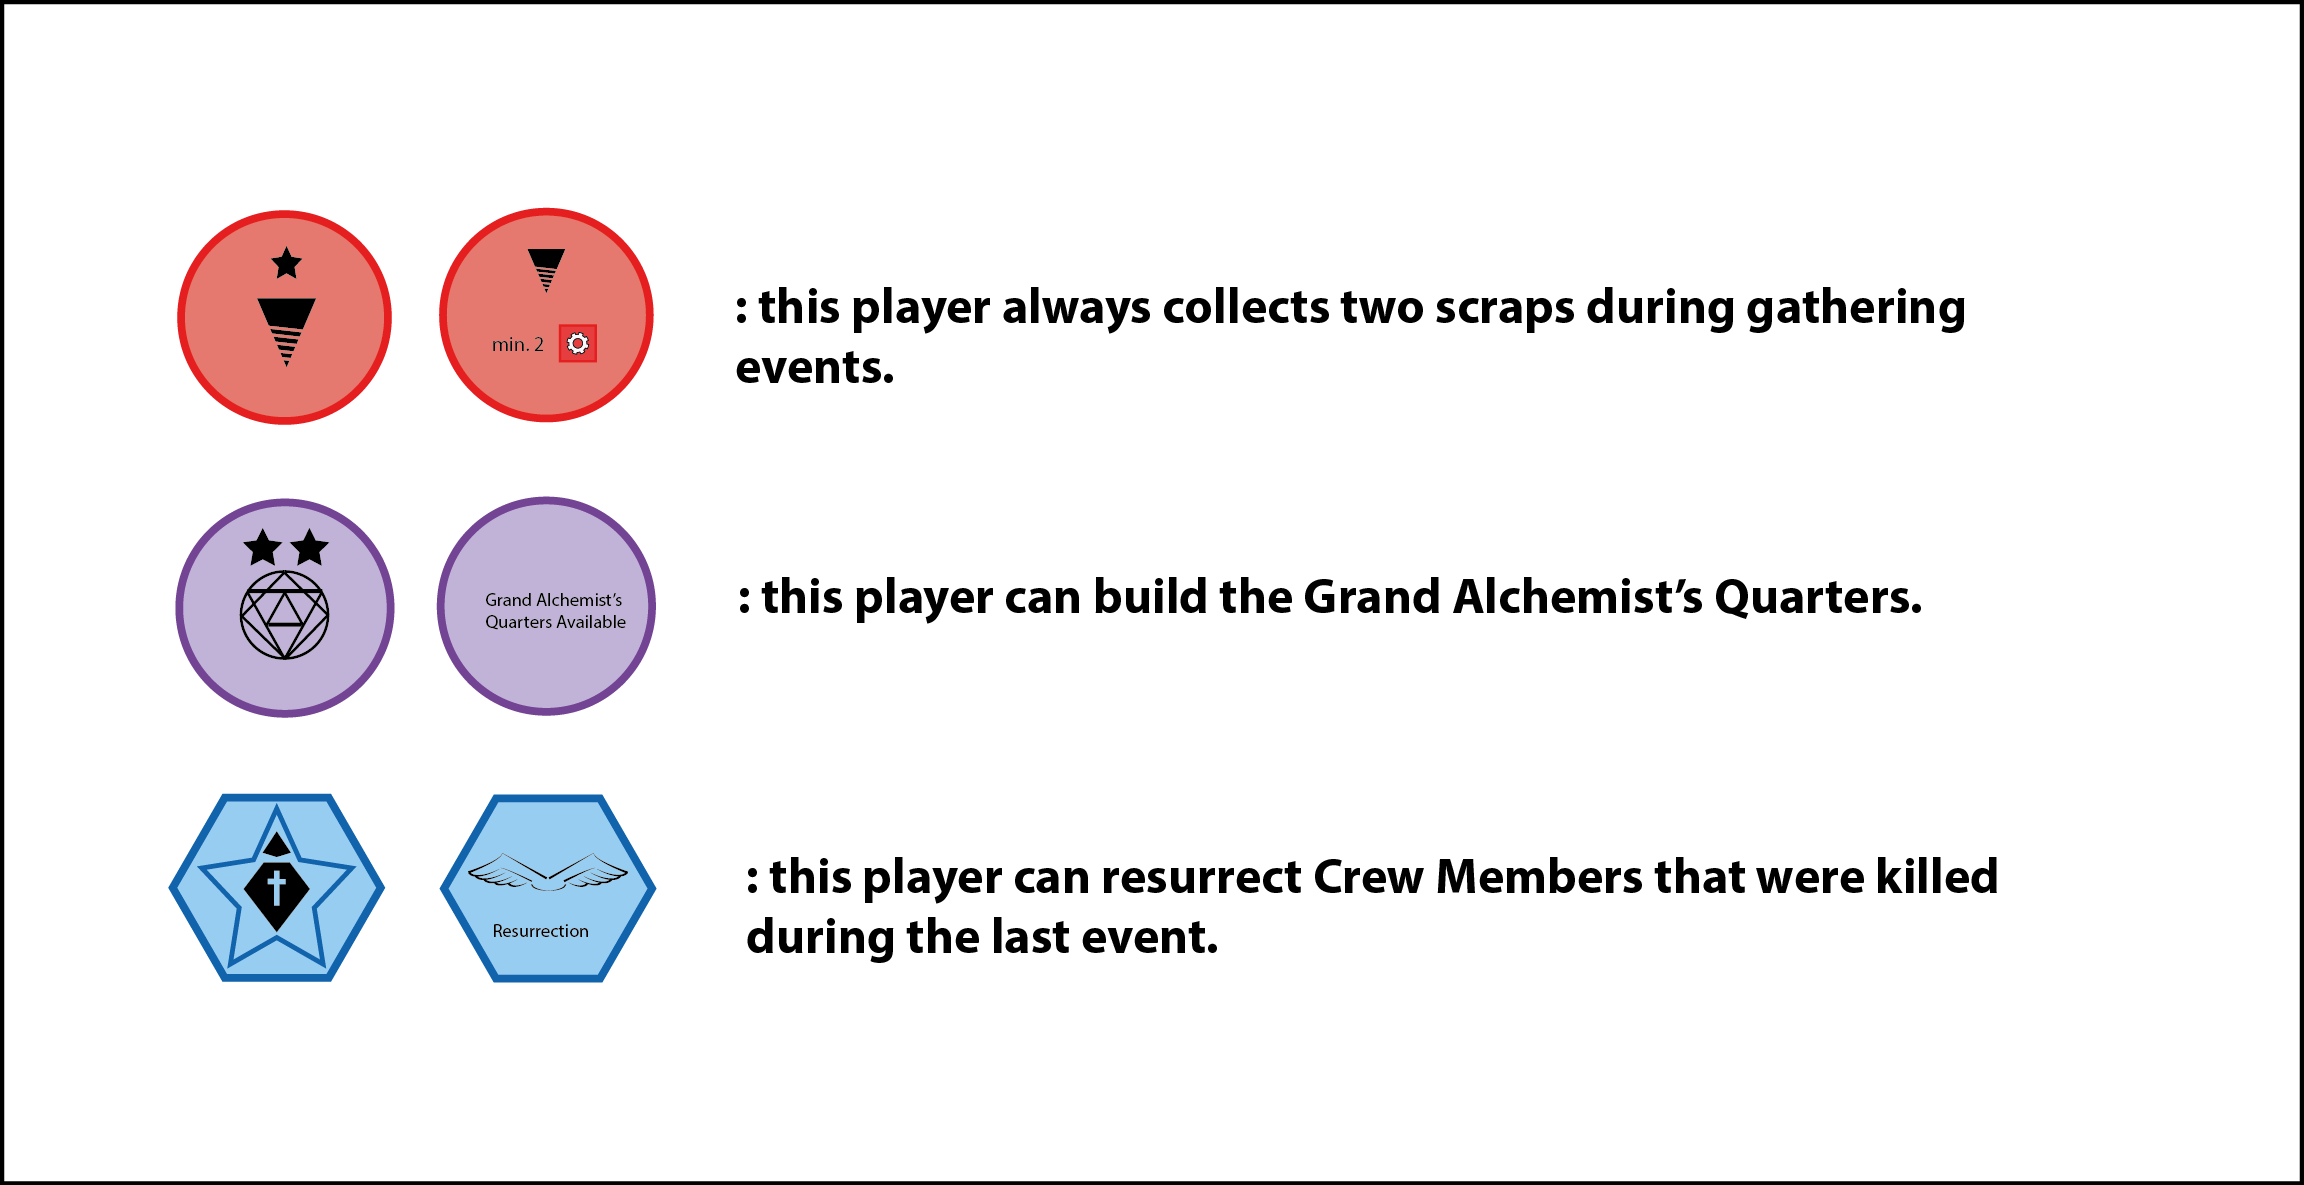
\includegraphics[width=\textwidth]{Images/Specialization.png}
    \caption{Examples of specialization tokens that players can have. Each of the tokens represents a bonus that can be useful when performing the procedurally generated events. The last token is the Priest's \textit{Mastery token}.}
    \label{fig:spec}
\end{figure}

The first type of \textit{Specialization token} grants a small bonus when visiting an island. The second type of \textit{Specialization token} always allow the player who has it to build the biggest rooms, called \textit{Mastery Rooms}. These rooms are not gained after merging. They are directly constructed for 8 \textit{Scrap} tokens, do not cost \textit{Alchemy Points} and require the castle's \textit{Crystal} to be powered at level 3. They take four construction spaces and grant the player the \textit{Mastery token} (see figure \ref{fig:temp}. This token provides important bonuses that affect the outcomes of the event.
 
\begin{figure}[!ht]
    \centering
    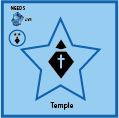
\includegraphics[scale=1]{Images/mastery.png}
    \caption{The Temple, that provides the priest's \textit{Mastery} token. The token allows the player to resurrect \textit{Crew Members} that died during an event for 1 \textit{Alchemy Point}.}
    \label{fig:temp}
\end{figure}

The bonus provided by the \textit{Mastery token} are very important, and the game can hardly be finished without them.

It is important to notice that the specialization tokens are only attributed to the first player who merges rooms of the same type. Therefore, two different players cannot have the same tokens.
\subsection{Phase 2 - Exploring the World}
\label{sec:p2}
When the first phase is over, and all the crew tokens have been assigned, the next phase is to explore the Archipelago.
As mentioned before, the first thing the players have to do in the world map, is to click on the reachable island they want to travel to. Once they have accepted to travel there, and have reached the location, the players will have to select a \textit{location} that they would like to explore.
Each area are connected to a type of resource, either it is a gathering area which will mainly yield building materials, or it is the research area which will yield mainly alchemy points. The players talk amongst themselves which one they would like to explore, and will have to choose based on what their current needs are. Once a location has been selected, the players will be presented with the event.

The player who is currently controlling the application reads out the event along with the possible options. It is now up to the players to talk amongst themselves to figure out which option they would like to pick. They also must decide which player should send a \textit{Crew Member}, according to which player is specialized. Also, the players have to remember that a \textit{Crew Member} can die in the process. The first class option is usually just sending a member of the crew down to complete the event, but there can be other options as well. The second class option adds a resource to the condition. It can be any of the four resources used in the game. The third class option requires a specialization token. In this case, it is the player that has the token that must send one of her \textit{Crew Member}. 

After the players have reached their conclusion and selected their option, the application will present them with the resulting outcomes of the event. It might be that they have lost a player token, gained one, a room has been destroyed, or simply that they got some resources. The outcomes vary. When the players have received their rewards and applied the results to the board, the players go back to the \textit{Management Phase}.

\subsection{Clean-up and start a new turn}
When returning from an event, all the pieces that were used the previous round, i.e. the crew tokens used for construction, the tokens assigned to the rooms, and the tokens used in the events, are returned to the players, and the board is cleaned up.
If an event yielded too much resources so that the cargo hold of the castle would be overfilled, it is up to the players to discuss which they would like to keep, and which to discard, before going back to phase 1 - management.
When this is done, the game repeats as described above with phase 1 and 2 and back again.

\subsection{Special Events}

Somewhere along the game, the players will most likely encounter the \textit{Special Events}. There are as of right now, two types of special events.

The first type is the fighting event. When this event occurs, the players will be presented with a scenario where two of the factions within the game, are fighting each other. It is then up to the players to decide whether they want to leave them alone, or if they would like to assist them. If they want to assist them, they have to choose their side. If the players are already friendly with one of the factions, they might want to assist that faction again. This choice is completely up to the players.

The other event type is memory based. It is an event that is based on previous events that the players have completed. The event is special in that it is based on previous data. For example, if the players visited an island controlled by the Highbournes, and they used some special healing on one of the options, then the special event could say something like "The highbournes saw you at the island, and want to learn how to use your healing magic". It is then up to the players to decide whether or not they want to help them, or not. Keeping in mind that their current standing with the faction will influence the outcome of whatever option they choose. 

\subsection{Winning or losing}
At one specific point on the map, there is a goal island. This island is the one the arrow is pointing towards, and is the one that the players are supposed to head towards in order to complete the game, and win.
If the players are able to reach this island, the game is over. The players will be presented with an ending screen in the application, and then they can choose to start a new game if they so choose. 

There are a number of different ways to lose the game. Since it is a collaborative game, if one of the players manages to get all his or her crew tokens killed, the game is over. Every player must have at least one crew token, in order for the game to still be in play.
Should the castle run out of crystal charges, the game will be over as well, as this would mean that the castle would be stuck floating in space and not be able to move.

\section{Last Playtest}
The prototype described above is the last one that was built during this prototype. It is the result of the combination of the game mechanics created for the purpose of experimenting hybrid games and the implementation of PCG to create a new kind of play experience.
\subsection{Modifications for testing purposes}
Earlier prototypes showed that the game was not ready to provide relevant results about its experimental purpose. Therefore it was decided to alter the prototype with a few modifications in order to obtain the necessary results. The players were intentionally left unaware of some of the modifications.

\subsubsection{Map layout and goal}
Originally, the map should have introduced a mechanic based on \textit{interest points}. The players should not have to only reach the final island on the map to win the game, but explore the Archipelago in order to find three specific islands before going to the final island. This mechanic was not implemented in the final playtest, as visual assets providing feedback were not ready at the moment of the playtest.

It was decided to simulate it by manually designating the next island to reach. This would not perfectly reproduce the intended experience, but at least it would simulate the feeling of exploration by forcing the players to explore a larger amount of islands.

\subsubsection{Special events occurrences}
The special events were a difficult part of the design of the game. It was necessary to have them occurring not too often, so they would always be unpredictable for the players. This is also why they have such particular parameters to be triggered. However, internal tests performed before the final playtest with players showed that the events were not occurring often enough. 

Since analysing the reaction of the players when facing a special event, it was decided that some regular events would be pre-made and set to occur at a given turn. To do so, the island would also be set to only generate one location during this turn. Also, two out of the three options offered in the event included in that location would trigger a special event, which would ensure that the players would have to go through it before moving on to the next island. The special events were set to be triggered at least once between each intermediary islands.

\subsubsection{Using a portable device}
After these modifications, the application was ready to provide relevant data. However, there was a last problem that would alter the data too much to be ignored. This experiment was supposed to test hybrid games as tabletop games using a digital component to enhance its gameplay. Throughout the development of the game, the application was running on a Personal Computer during playtests. It was important for the final playtest to be able to use a smartphone or a tablet as a digital component. This would allow us to gather data of better quality about how intrusive the digital component is in the flow of hybrid games.  
Since the original development of the application had been towards a Personal Computer, the scale of all the UI elements were off when it was built to the tablet device. Everything was scaled down and was super small and the text were unreadable. This meant that the elements needed to be enlarged in order to properly supply the users with the wanted looks. At the time of the actual play test, the layout of the application was significantly enlarged, and all the elements were manually fitted to make sure that the players would experience the application in the best possible way, so that the looks of the elements would not hinder the actual gameplay experience.

\subsection{Material, Scope and resolution}
The \textit{Material} of the prototype was closer of what players would expect when playing a hybrid game. It was the first time that the game was tested with analogue components made of something than paper, thus changing the tactility of the different pieces. With earlier prototypes using paper to iterate more quickly, the players had shown frustration when not being able to pick up the bits of paper, or losing them. Using cardboard for the tokens would ensure that this problem would not alter the results. As explained above, the digital component was a tablet for the first time. This would help providing the necessary information related to the flow of the game. However, since the port to tablet was made in a very brief time, some problems with zooming as well as fluidity drops when moving the camera around on the map would alter the experience. This problem was explained to the players prior to testing, and taken into account in the final results.

This is the highest fidelity prototype that was created during this project. Although all the visual assets are still place-holders, the prototype uses a tablet as a digital device and that all the mechanics are implemented. 

It is the first time the \textit{faction} system and the special events are introduced in the game, and are not tested separately. Therefore, testing those mechanics is the main purpose of the prototype. By testing these two new elements and how they fit in the game, the \textit{Scope} of this prototype covers all the principles previously mentioned all along this paper. About the game itself, a progression in the difficulty must be visible when the players reach the intermediary islands. The difficulty must increase, and the decisions should be taken more carefully. Also, the players must realize that their choices have influenced the game and the generation of content. Finally, the specialization must be strong enough so that the players construct their authority in the game. 

\subsection{The Playtest}
The descriptions established in the following paragraphs are based on a transcription of notes taken during the playtest (see appendix \ref{sec:transcript}). After the game, some questions were asked to the testers during a short interview. This interview was conducted in the form of an open discussion, guided by a few general questions. The observation and the interview were audio-recorded, but the playtesters did not give their authorization to join the recording in this paper. Therefore it is not included, but a transcript of the notes taken has been included as an appendix (the names of the testers have been changed). The observers from the development team were the designer of the game and one of the two programmers.
\subsubsection{Preparation of the playtest}
The playtest has been organized in a place that all the testers know. The testers are three game design students who all have  some experience with tabletop games (mostly trading card games). Two of the people chosen, had never seen the game before. They are the beginners to who the third playtester has to teach the rules. The third playtester is the only one that has experienced with a previous version of the game: if the specialization system is not strong enough, that player would take a \textit{leader}'s role - which is not wanted. The playtest will start in the normal starting conditions of the game.

The players are informed that the application is not completely ready, and that they will have troubles moving the camera around in the map screen. They are informed of the other modifications made to the prototype, except those about the special events occurence. Those decisions were taken so that their reactions are as natural as possible when playing.

The game being a hybrid board game, the players have been informed that they could ask questions to the observers in case they could not find the solution of a problem in the rules. If the observers think that the question is legit and the answer is hard to find in the rules, they decide to give that information and take notes about how to solve the problem. 

\subsubsection{Observation process and data gathering}
During the observation, notes relevant to the scope of the prototype were taken following the game flow. Not all the actions performed by the players would be transcribed as notes, as the quantity of data to sort after the playtest would be too overwhelming. It was decided that only important elements of the game session would be noted. Listening to the audio record would then provide the missing details.

The focus points of the notes were

\subsection{Feedback and results}
The observations made during the playtest, as well as the open discussion with the testers showed both the successes and failures of \textit{Archipelago} in the state it was as a final prototype. The results will be classified according to the main aspects that \textit{Archipelago} should cover, as described in section \ref{sec:dev}.

\subsubsection{Specialization and collaboration}
The core loop was the first element that was prototyped during development. Early results showed that this core loop provided a solid base for discussion and could allow the integration of a digital component to base the \textit{Exploration phase}. The collaboration system as it is in the final prototype reinforced that feeling. The decisions were based on the available resources and more generally on the status of the team. Using \textit{Crew Members} to divide the action points between players provided interesting results. As noticeable during the playtest, a large part of the discussions were based on who should save a \textit{Crew Member} during the \textit{Management phase} to use it in order to perfom events. This changed the strategy a few times, as some rooms could not be built because of that. This altered the decisions to take during events, and showed the potential of using collaborative gameplay in a PCG based game.

The system of specialization however, did not provide the intended results. Although the playtesters seemed to enjoy having to construct the specialization by themselves, the bonuses were not useful enough in the mechanics of the game. After the players realised that, the only motivation for them to get the tokens was just the satisfaction of knowing that they had powers that the others did not have. More generally, the bonuses attributed thanks to the tokens need to be reworked to correctly fit with the rewards gathered during the events. Also, the specialization should have forced the players to have the authority in a particular field. However, the limited possibilities of actions to perform during the \textit{Management phase} did not emphasize this need for specialization. In general, there was no need to discuss it, and the player specialized in one field would naturally take the decision by himself.

\subsubsection{Event Generation system}
The standard event generation system provided interesting results. First of all, the parameters used to generate the events were sufficient.
The faction system and the special events must support the core mechanics and provide a particular feel. Indeed, one of the interests of using PCG to support board game mechanics is to reuse the players input in order to pass them as parameters to generate content. The players should notice this and understand how their actions influenced the game content generation. 

During the playtest, it first appeared that the players did not notice at once that they triggered a special event. And when they did, they did not realise that this event was based on actions that they performed earlier. After the second special event however, one of the playtesters realised that the faction followed them from a previously visited island. But the name of the island was too abstract to remind them what they did to trigger the faction's reaction. User Interface elements did not provide the necessary information to remind the players what part of the content had been affected by the results. 

The events themselves, and the content represented within them in terms of the flavour text for the event and the options within it, were well received. The events are able to convey efficiently to the players what is going on and what the players have to do in order to complete the events. 
In the first few events that were engaged during this playtest, the playtesters did not really take notice of how the event options were combined, and had to read the text out loud more than once, in order to fully understand what needed to be done. But as the game progressed, the playtesters started noticing the signifiers more clearly. By this, the signifiers specifically mean the token indicators next to the option text on the events.

When the playtesters had started to get a good feel for how the events were presented, and how to quickly read them, they started talking more about why they should pick one option over the other, and generally opened up the game for more conversation and collaboration within the team.

\subsubsection{Theme and Narrative}
There is obviously a lack of depth in \textit{Archipelago}'s narrative. However, the playtest showed how this question should be tackled in later iterations.
\subsubsection{Device integration}
The feedback received from the playtesters showed that using the application was an important and interesting part of the game experience as a whole. The players wanted to have the device in the hands to perform the actions. However, a problem that was noticed was that it is a bit confusing to not have a dedicated player that uses the device as it is the case in some other hybrid games. The testers were confused about who should have the application in the hands. Also, having one of the players reading out loud while the others are listening showed problems of engagement: some players were only listening to the outcomes, letting the other players do the rest of the actions.

They did, however, also note that the interaction with the app was at some points a bit much, as the screen was relatively small, which made the text a bit hard to read if the flavour was large. They did also note that this was to be expected as this was a playtest of a prototype, and that the finished product would be different. The playtesters also gave the feedback that it could be nice, if the text was too small, to have some sort of button that would allow the text to be read out to the players. This way, they would not have to read it out to themselves, but could instead listen as a group.


The playtest showed that the game in its current has too many flaws to be enjoyable as a satisfying hybrid game experience. However, the results encountered thanks to playtesting, as well as the whole development procedure revealed interesting that should be discussed in the context of the previously established framework.